%!TEX root = ../main.tex
%
% オシロスコープ
%

\section{オシロスコープ}

\subsection{オシロスコープとは}

オシロスコープは、画面の横軸を時間、縦軸を電圧として、電圧の時間変化を表示する装置です。従って、電圧が一定であるようなDC(直流)の場合は
横に延びた時間変動のない直線が表示され、AC(交流)の場合は電圧が周期的に変化するグラフが表示されます。

オシロスコープを用いれば、非常に短い時間の電圧変化を捉えることができ、他の装置と組み合わせることによって様々な測定に用いたり、
電気回路の特性を調べたりすることができます。

%オシロスコープは、電気信号の波形観測を行うための測定器です。これによって、交流電流など、電気信号の時間的変化を観測することができます。もちろん、直流電流の電圧を測定することも可能です。

ここでは、2つの電気信号を入力し観測することができる2現象オシロスコープの使い方を学び、交流信号の周期や周波数を求めると同時に、波の合成について学習しましょう。




\subsection{基本的な動作}

オシロスコープにはブラウン管を使ったタイプのものや、
信号をデジタル的に処理して液晶ディスプレイに表示するタイプのものなど
様々な種類があります。
古くはブラウン管を使ったものが主流でしたが、電気回路が半導体などのデジタル素子を使っているものが
主流となったため、アナログ信号をデジタル信号に変換(A/D変換)して処理するものが多くなっています。

今回の実験で用いるオシロスコープ(PicoScope)は、
外部装置側で電圧をA/D変換してメモリに蓄積し、
デジタル処理されたデータをUSBインターフェイスを通じてパソコン側のソフトウェアで読み取り、表示するタイプのものです。
このタイプのオシロスコープは、処理の一部と表示(液晶ディスプレイ)をパソコンで行うため価格を比較的抑えることができる
利点がありますが、
パソコンやUSB通信の処理速度を超えた信号変化には追随できないという欠点があります。


\begin{enumerate}

\item オシロスコープの使い方

\begin{itemize}

\item パソコンとUSBケーブルを使って接続する。

\item デスクトップのアイコンをダブルクリックして、オシロスコープ用ソフトウェア「PicoScope 7 T\&M」を起動する。

%\item みの虫クリップ付きBNCケーブルを接続する。(チャンネルAまたはB)

\item みの虫クリップ付きケーブルなどを使って、チャンネルAまたはBのBNCコネクタに発振器もしくはマイクを接続する。

\item 「トリガー」をクリックし、モードを「なし」に設定する。

%\item サンプル数を「100 kS」、入力レンジを「自動」、カップリングを「DC」に設定する。

\item 入力チャンネルAまたはBをクリックし、入力レンジを「自動」、カップリングを「DC」に設定する。(使用しないチャンネルは「オフ」にする。)

\item 画面上部の「Scope」に「+/-」ボタンを使って、タイムベース(横軸の1目盛が表す時間)をセットする。
(音叉や音声を測定する場合には1 [ms/div]〜5 [ms/div]の値にセットする。)

%\item うまく波形が出ない場合は、発振器や音を流した状態で「AUTOSET」を押して調整する。

\item うまく波形が出たら、「スペースキー」または「実行/停止ボタン」を押して画面を固定する。

\item 印刷メニューから波形を印刷する。

\item リサジュー図形(XY表示)は、画面上部の「計測」をクリックし、「XY」を選択することで表示できる。
その際、タイムベースを5 [ms/div]に設定する。

\end{itemize}

\item 発振器の使い方

\begin{itemize}

\item コンセントにつなぎ、右下の電源スイッチを入れる。

\item 「減衰器(ATTENUATOR)」を-20 [dB]、「振幅(AMPLITUDE)」ダイヤルを真ん中あたりに設定する。

\item ダイアルと右のボタンの倍率を組み合わせて、出力周波数を100 [Hz]に設定する。


\end{itemize}


\end{enumerate}


\newpage

\subsection{リサジュー図形を見る}

基本の動作では、各チャンネルに入れた信号を、横軸に時間、縦軸に電圧をとって 
表示させましたが、2現象オシロスコープでは、2つのチャンネルに入力された信号を、 片方は縦軸に電圧をとり、もう一方は横軸に電圧をとって、合成して表示することも可能です。この時に現れる図形をリサジュー図形といいます。
%この場合は、軸の調整は、縦軸、横軸共に電圧(Volts/div)のダイヤルで行います。


リサジュー図形を見ることによって、二つの電気信号の周波数の比率、位相の差を 
測定することができます。$\Rightarrow${\bf [実験 5-2]}

\begin{center}
\begin{tabular}{c|ccccc}
& \multicolumn{5}{c}{位相差} \\
周波数比 & $0^\circ$ & $45^\circ$ & $90^\circ$ & $135^\circ$ & $180^\circ$ \\
\hline
\begin{minipage}[b]{5mm}
1:1\\
\end{minipage} &
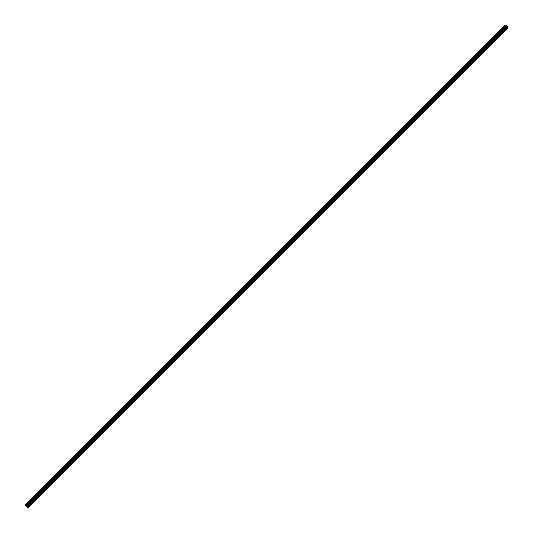
\includegraphics[scale=0.2]{05_Oscilloscope/1-1.eps} &

\includegraphics[scale=0.2]{05_Oscilloscope/1-2.eps} &
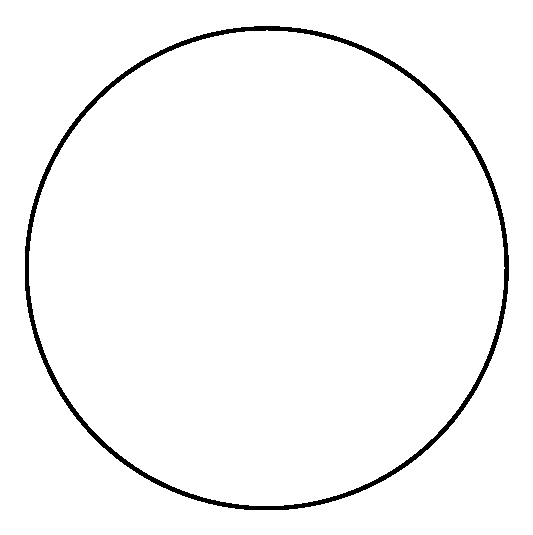
\includegraphics[scale=0.2]{05_Oscilloscope/1-3.eps} &
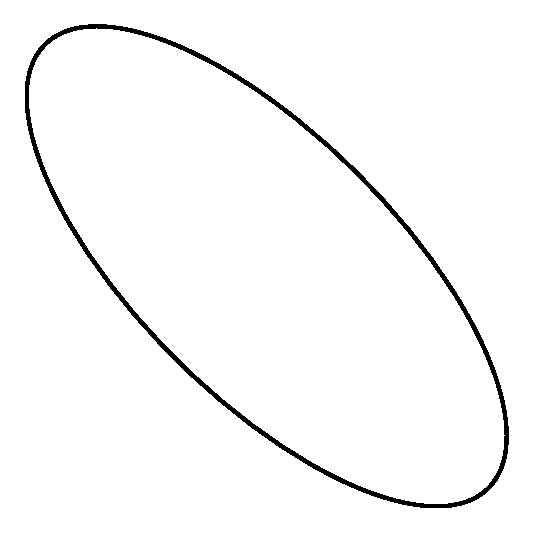
\includegraphics[scale=0.2]{05_Oscilloscope/1-4.eps} &
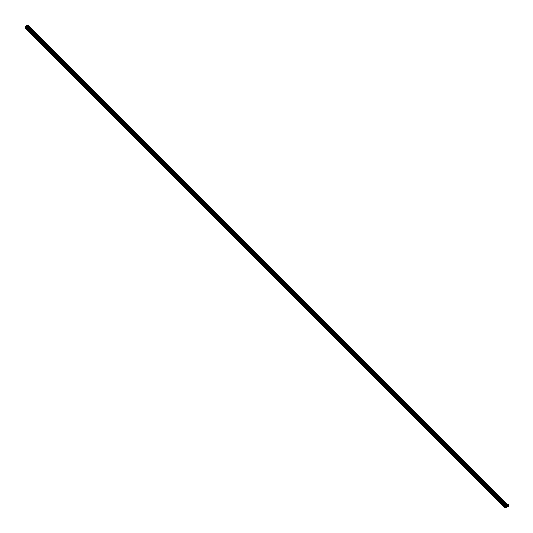
\includegraphics[scale=0.2]{05_Oscilloscope/1-5.eps} \\
&&&&&\\
\begin{minipage}[b]{5mm}
1:2\\
\end{minipage} &
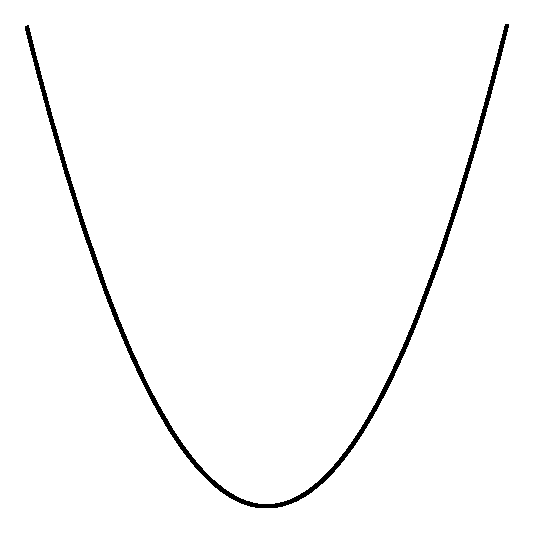
\includegraphics[scale=0.2]{05_Oscilloscope/2-1.eps} &
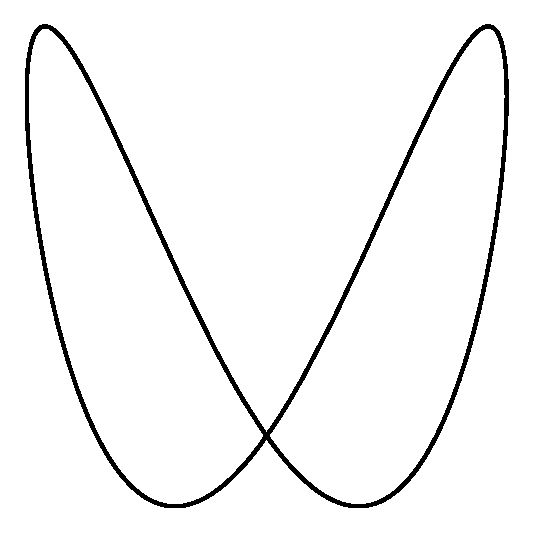
\includegraphics[scale=0.2]{05_Oscilloscope/2-2.eps} &
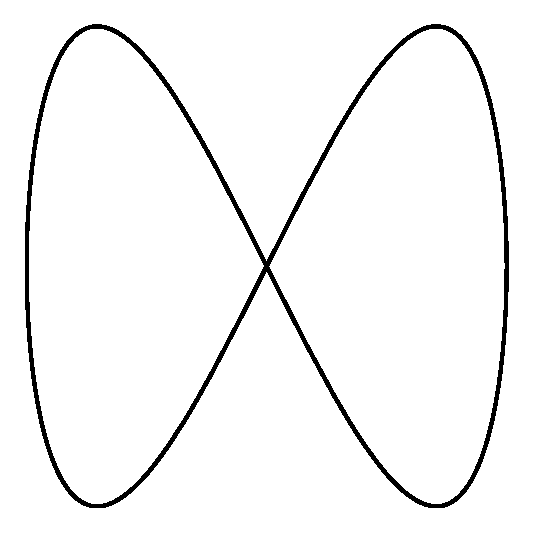
\includegraphics[scale=0.2]{05_Oscilloscope/2-3.eps} &
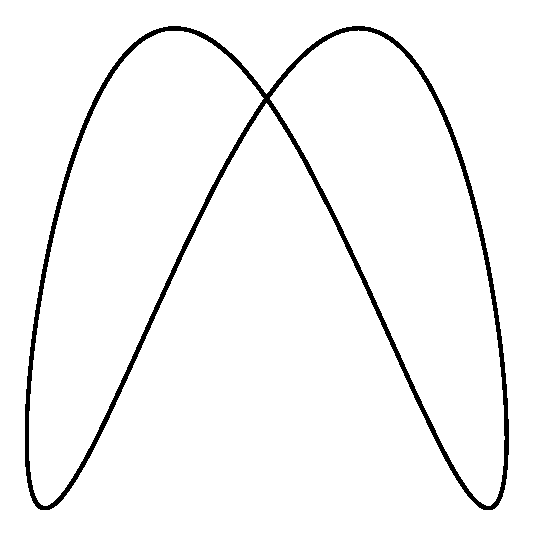
\includegraphics[scale=0.2]{05_Oscilloscope/2-4.eps} &
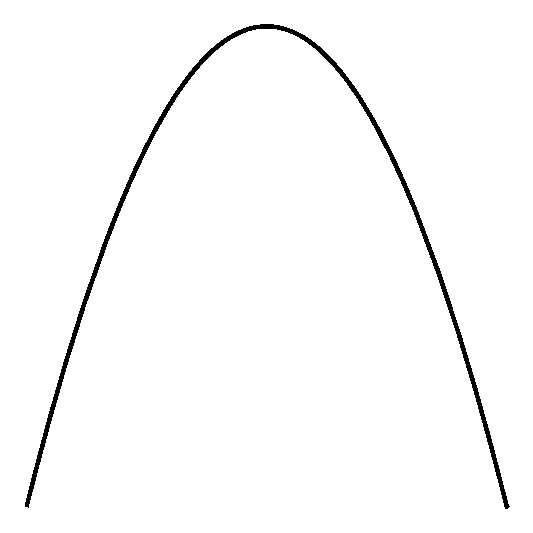
\includegraphics[scale=0.2]{05_Oscilloscope/2-5.eps} \\
&&&&&\\
\begin{minipage}[b]{5mm}
1:3\\
\end{minipage} &
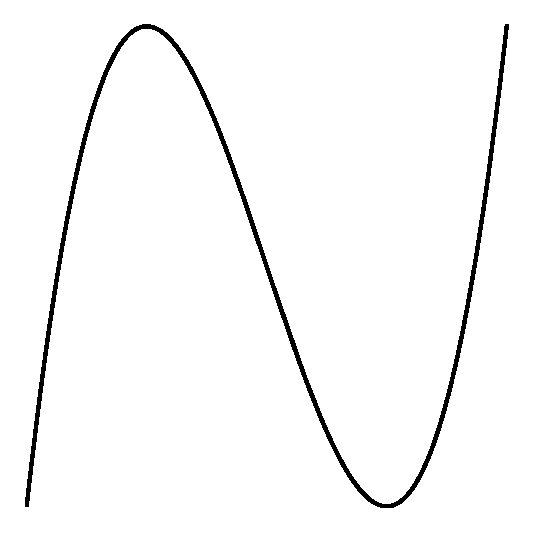
\includegraphics[scale=0.2]{05_Oscilloscope/3-1.eps} &
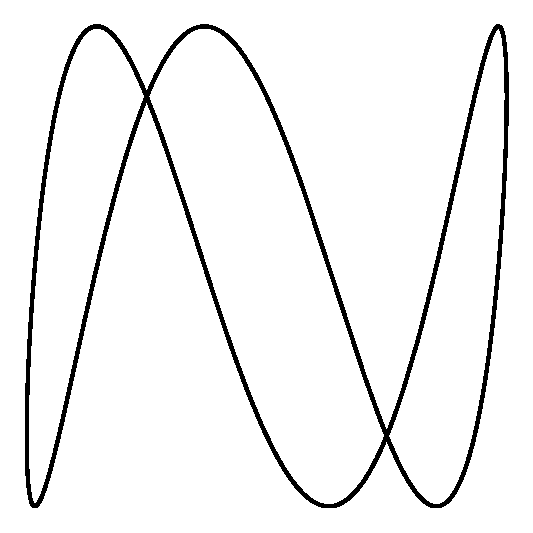
\includegraphics[scale=0.2]{05_Oscilloscope/3-2.eps} &
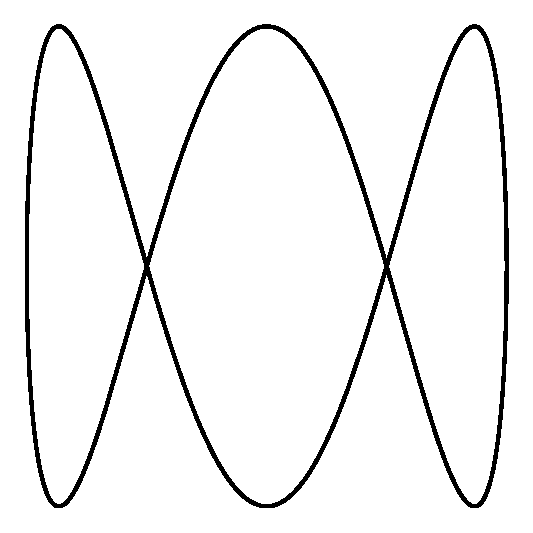
\includegraphics[scale=0.2]{05_Oscilloscope/3-3.eps} &
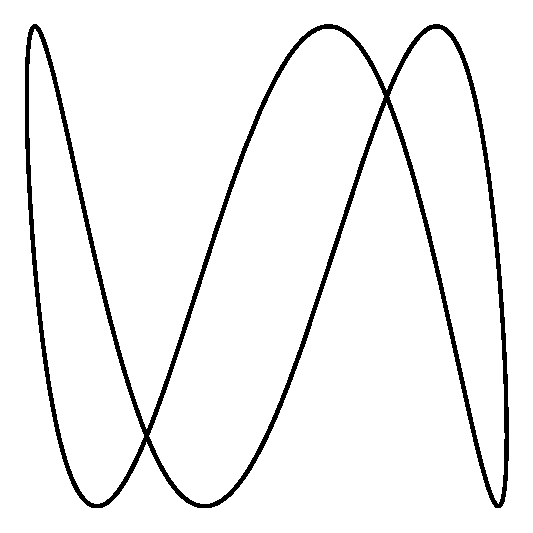
\includegraphics[scale=0.2]{05_Oscilloscope/3-4.eps} &
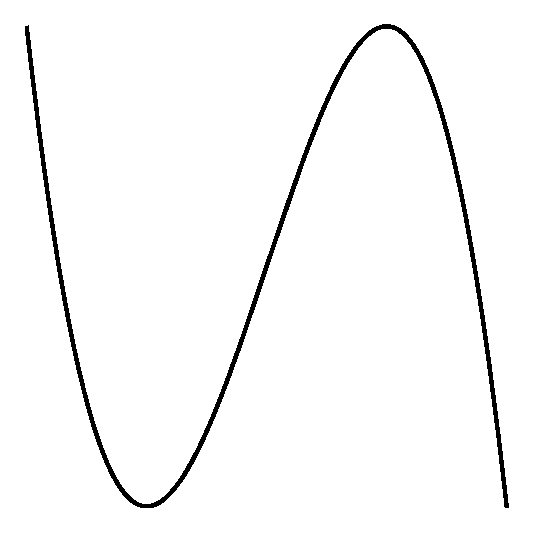
\includegraphics[scale=0.2]{05_Oscilloscope/3-5.eps} \\
&&&&&\\
\begin{minipage}[b]{5mm}
2:3\\
\end{minipage} &

\includegraphics[scale=0.2]{05_Oscilloscope/4-1.eps} &
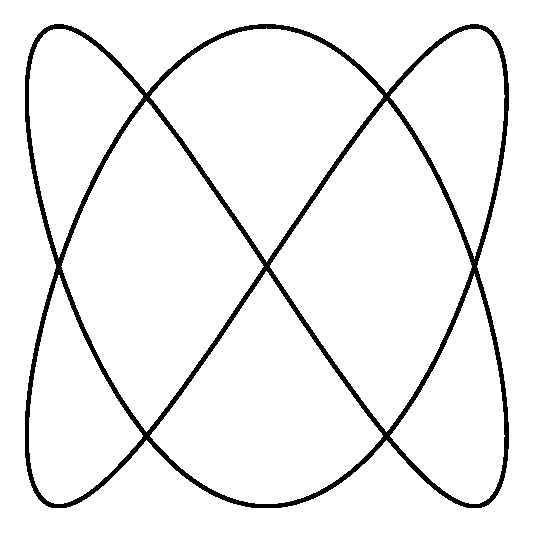
\includegraphics[scale=0.2]{05_Oscilloscope/4-2.eps} &

\includegraphics[scale=0.2]{05_Oscilloscope/4-3.eps} &
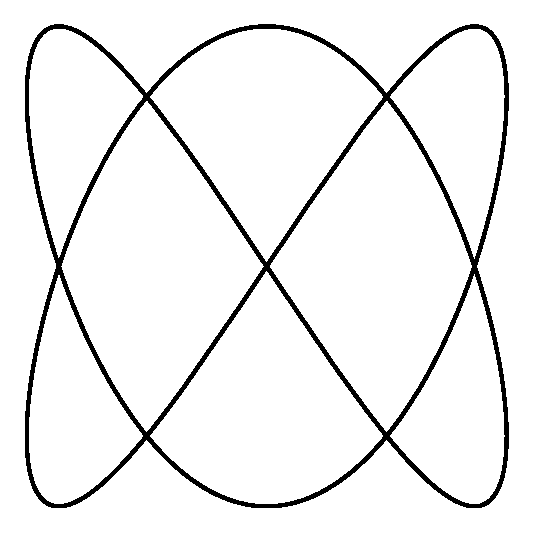
\includegraphics[scale=0.2]{05_Oscilloscope/4-4.eps} &

\includegraphics[scale=0.2]{05_Oscilloscope/4-5.eps} \\
\end{tabular}
\end{center}

\newpage

\jikken

\begin{itemsquarebox}[c]{\bf 実験用具}
2現象オシロスコープ、発振器2台、音叉、マイク、 
みの虫クリップ付きBNCケーブル 
\end{itemsquarebox}

\bigskip

\subjikken{1つの波形の観察}

\begin{enumerate}

\item 発振器からの100 [Hz]の正弦波を、オシロスコープのチャンネルAに入
力し、波形を観察しましょう。また、パソコンに表示された波形のデータを印刷します。波形から、波の周期:$T$ [s]を読
み取り、$\nu=1/T$より、波の周波数を求めることができます。入力信号の周波
数を計算し、100 [Hz]になっていることを確かめましょう。

\item マイクをオシロスコープのチャンネルAにつなぎます。
マイクの前で音叉をたたき、音波の波形がオシロスコープの画面に表示さ
れることを確かめます。次に、マイクに向かって声を出し、声の波形を
表示させ観察しましょう。
波形のデータを印刷したものから、この声の周期$T$ [s]を読み取
り、自分達の声の周波数を求めてみましょう。

\item 周波数がわずかに異なる2個の音叉を同時にたたいてうなりを発生させ、
オシロスコープでその波形を観察してみましょう。
(うなりが見えるように「収集時間」を調整する必要があります。)
また、オシロスコープの表示画面からうなりの振動数を
求めてみましょう。(音叉の振動部分におもりを取り付けることで振動数をずらすことができます。)
2個の音叉それぞれの振動数とうなりの振動数の間にはどのような関係があるでしょうか。

※ マイクは音叉の共鳴箱の開口部に近づけると大きな音を拾うことができます。

\end{enumerate}


\subjikken{リサジュー図形の観察と音叉の周波数の測定}

\begin{enumerate}

\item 2台の発振器から同じ周波数の信号(100 [Hz]でよい)をチャンネルA、チャンネルBに入力し、XY表示に切り替えて、チャンネルAとチャンネルBの波の大きさが大体同じになるように「入力レンジ」を調整します。
また、図形が流れたり動く時は発信器の周波数を微調整します。

\item 表示されたリサジュー図形を観察しましょう。また、
そのまま通常の表示(横軸が時間)に切り替えて、同様に記録し、2つの波形の
位相のずれを観察し、リサジュー図形の形と照らし合わせてみましょう。

\item 同様に、発振器からの信号が1:2のときと、1:3のとき(100 [Hz]と200[Hz]、 
100 [Hz]と300 [Hz]でよい)についてもリサジュー図形を表示させ、
リサジュー図形と2つの波形を比較しましょう。
(プリンターで印刷して比較しても良い。)

\item 次に、リサジュー図形を利用して、音叉の周波数を測定してみましょう。チャンネルAに
はマイクをつなぎ、チャンネルBは発振器をつないだままにし
て、マイクの前で音叉をたたきます。発振器の周波数を変えて、1:1の周波数
の場合のリサジュー図形が表示されるところを探し、音叉の周波数を求めましょ
う。


\end{enumerate}

